\chapter{Interaktionsdesign}
%In diesem Abschnitt soll analysiert werden, wie die möglichen Interaktionen gestaltet sind. %Werden die Designprinzipien Normans (Kap. \ref{sec:interactionDesign}) nicht hinreichend erfüllt, lässt dies auf ein zu behebendes Problem der User-Experience schließen.
Da es sich bei dem System um eine bestehende Anwendung in der Entwicklungsphase handelt, ist bereits ein Interaktionskonzept vorhanden. Dieses wird im Folgenden analysiert und erläutert, um eine Orientierung zu ermöglichen. Spezielle Designentscheidungen werden dabei hervorgehoben. Das Hauptaugenmerk dieses Abschnittes wird auf der Entwicklung alternativer Eingabemethoden liegen, die es dem Nutzer ermöglichen sollen, die vorhandenen Interaktionen intuitiver und mit dem Eingabegerät seiner Wahl durchführen zu können. Zudem wird die Anwendung auf eine Benutzung an Tablet-PCs und anderen Geräten mit Touch-Bedienbarkeit, wie z.B. Convertibles, vorbereitet. Convertibles sind Computer, die sowohl als Laptop, als auch als Tablet genutzt werden können.\par
\section{Analyse}
%Die Anwendung besteht im Wesentlichen aus drei UI-Bereichen. Der erste Bereich ist die \textbf{Navigation}, die sich am oberen Rand des Fensters befindet. Hier werden zusätzlich zu den Navigationselementen Hilfetexte eingeblendet. Das zweite Areal, genannt \textbf{Sidebar}, ist an der rechten Seite der Applikation untergebracht und stellt weitergehende Informationen und Interaktionsmöglichkeiten für den aktuell angezeigten Bildschirm zur Verfügung. Der letzte und größte Bereich ist der \textbf{Content}-Bereich. Er nimmt den übrig gebliebenen Platz ein. Hier werden die Hauptinformationen und -bedienelemente dargestellt.\par
\begin{figure}[H]
 \centering
 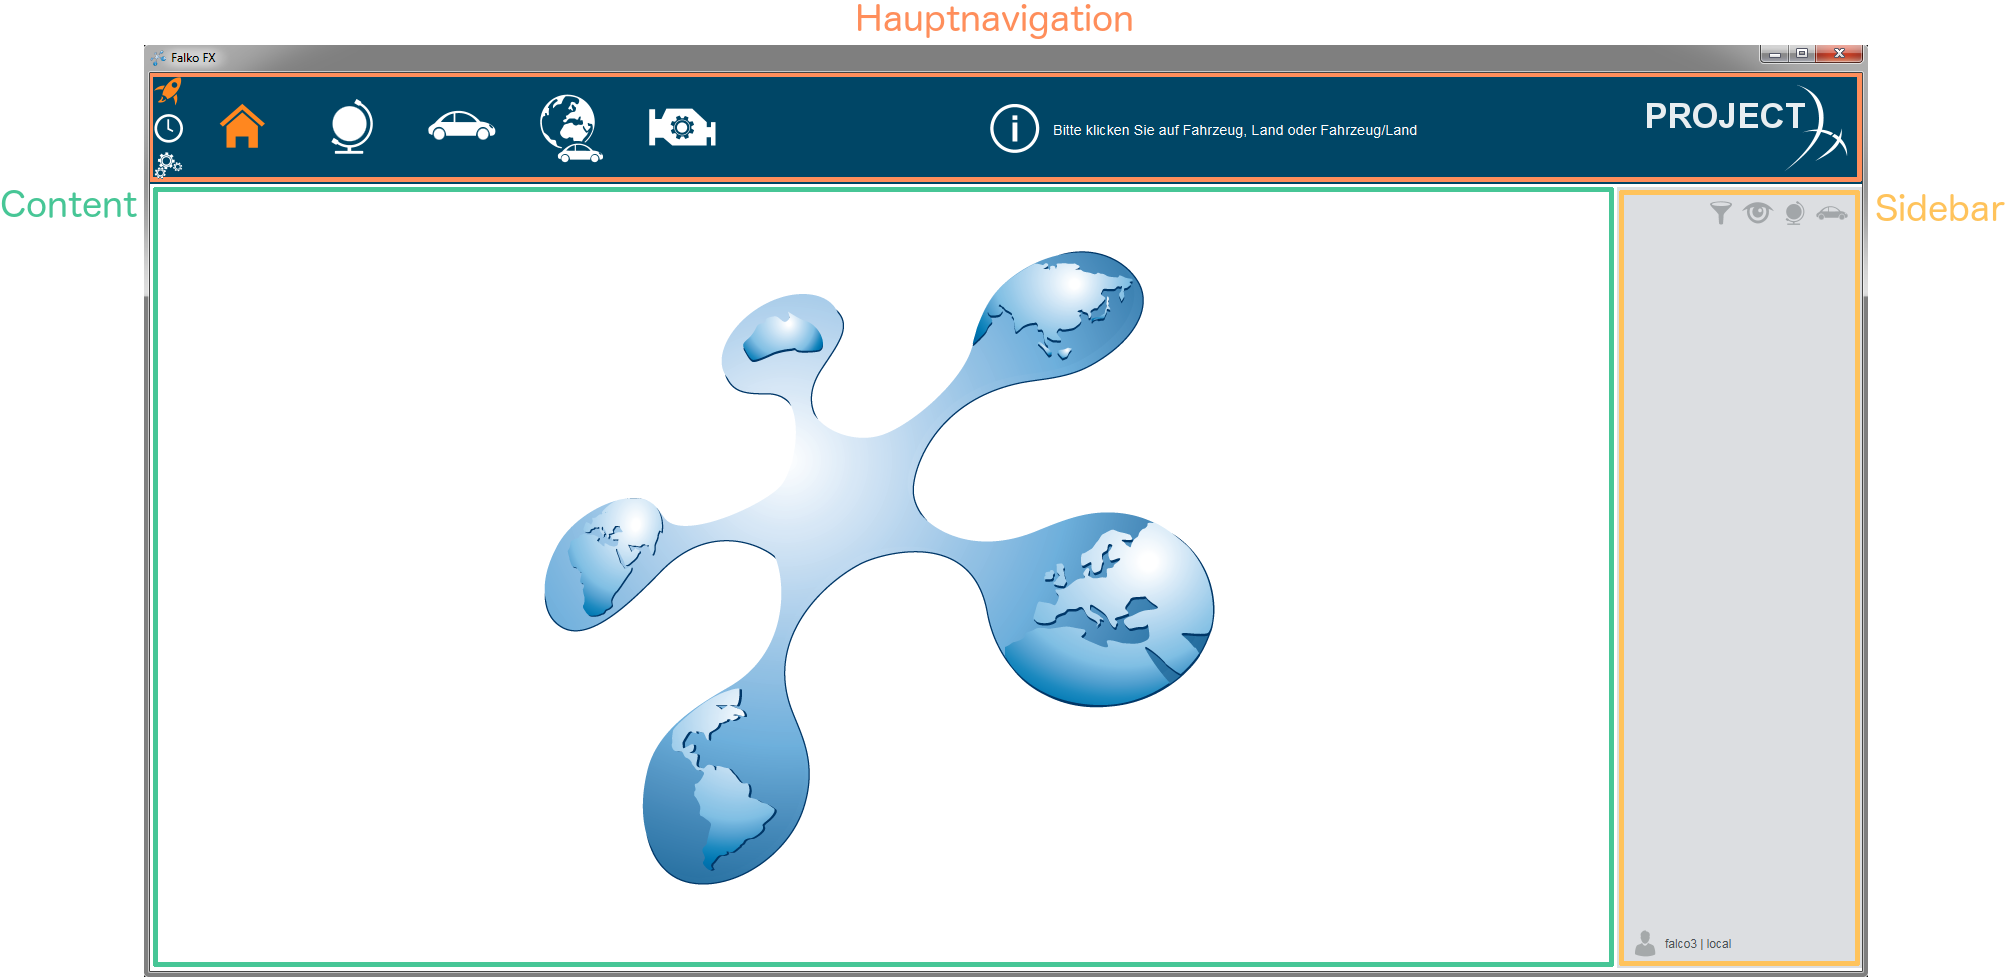
\includegraphics[width=0.9\textwidth]{grafiken/areas.png}
 \caption{Bereiche der Anwendung}
 \label{fig:areas}
\end{figure}
Das Konzept der gemeinsamen Region wird hier durch die verschiedenen Hintergrundfarben realisiert und unterstreicht die unterschiedlichen Funktionalitäten.\par
\heading{Navigation}
Im Navigationsbereich findet sich im initialen Zustand die Hauptnavigation wieder. Durch die Bedienelemente an der linken Seite der Leiste kann zwischen folgenden Funktionen gewechselt werden:
\begin{enumerate}
	\item Hauptnavigation: Wechsel zwischen Standard-Anwendungsfällen und der verschiedenen Ansichten
	\item Versionsvergleich: Navigation für Anwendungsfälle mit Versionsvergleich (derzeit in Entwicklung und daher nicht weiter betrachtet)
	\item Einstellungen: Menü zum Verwalten anwendungsspezifischer Einstellungen
\end{enumerate}
\begin{figure}[H]
 \centering
 
\includegraphics[width=0.05\textwidth]{grafiken/ribbon.png}
 \caption{Umschalten der Navigation}
 \label{fig:ribbon}
\end{figure}
Durch die vertikale Orientierung, der geringeren Größe und der Nähe zueinander heben sich die Elemente zum Umschalten der Navigation deutlich von den anderen Schaltflächen ab. Wird eines der Elemente angewählt, wird eine Aktion ausgeführt und die Kindelemente, falls vorhanden, werden mittels Animation sichtbar. Die nachfolgenden Elemente der höher liegenden Ebenen werden \enquote{zur Seite geschoben}.\par
\begin{figure}[H]
 \centering
 
\includegraphics[width=0.85\textwidth]{grafiken/navi.png}
 \caption{Navigationshierarchie}
 \label{fig:navi}
\end{figure}
Die Elemente einer einzigen Navigationsebene benötigen keine weitere Trennung, denn durch den ausreichenden Freiraum ist diese bereits gegeben. Zwischen den verschiedenen Ebenen wird zusätzlich zu einer Farbabstufung eine weiße Trennlinie eingeblendet, die auf der linken Seite einen angedeuteten Pfeil enthält, der die Navigationshierarchie verdeutlicht. Dazu trägt ebenfalls die bereits erwähnte Animation bei.\par
Das Piktogramm des selektierten Navigationselementes wird orange eingefärbt, um die Orientierung zu gewährleisten. Es genügt ein kurzer Blick auf die Navigationsleiste, um festzustellen, welcher Navigationspunkt angewählt ist, da das Element nach dem Gesetz der Prägnanz heraussticht. Kann der Nutzer eine bestimmte Interaktion nicht ausführen, erscheint das Icon erwartungsgemäß ausgegraut.\par
Durch das Anklicken eines Icons wird der neue Bildschirminhalt angezeigt. Dies geht oft mit dem Laden von Daten einher. Sollten Daten aus der Datenbank geladen werden müssen, wird währenddessen eine Ladeanimation angezeigt. Andernfalls wird die Oberfläche in weniger als 500 Millisekunden aktualisiert, wodurch kein weiteres Feedback von Nöten ist. Stattdessen würde eine kurz aufblitzende Ladeanimation den Anwender eher irritieren als unterstützen.\par
\subsection{Datenauswahl}
Den Einstieg in jeden Anwendungsfall bietet der Filter. Er wird angezeigt sobald das Anwendungsfall-Symbol aus der Navigationsleiste selektiert wurde. Der Filter besteht in der simpelsten Variante aus folgenden Komponenten:
\begin{itemize}
	\item \textbf{Radial-Menü:} Ein rundes Menü, in dem die zu filternden Attribute ausgewählt werden können
	\item \textbf{Multi-Level-Liste:} Eine mehrstufige Liste mit Suchfunktion, aus der Werte zu den Attributen angewählt werden können
	\item \textbf{Filterselektion:} Eine Liste, welche die aktuell ausgewählten Werte gruppiert darstellt und das Abwählen dieser Werte erlaubt
\end{itemize}
\begin{figure}[H]
 \centering
 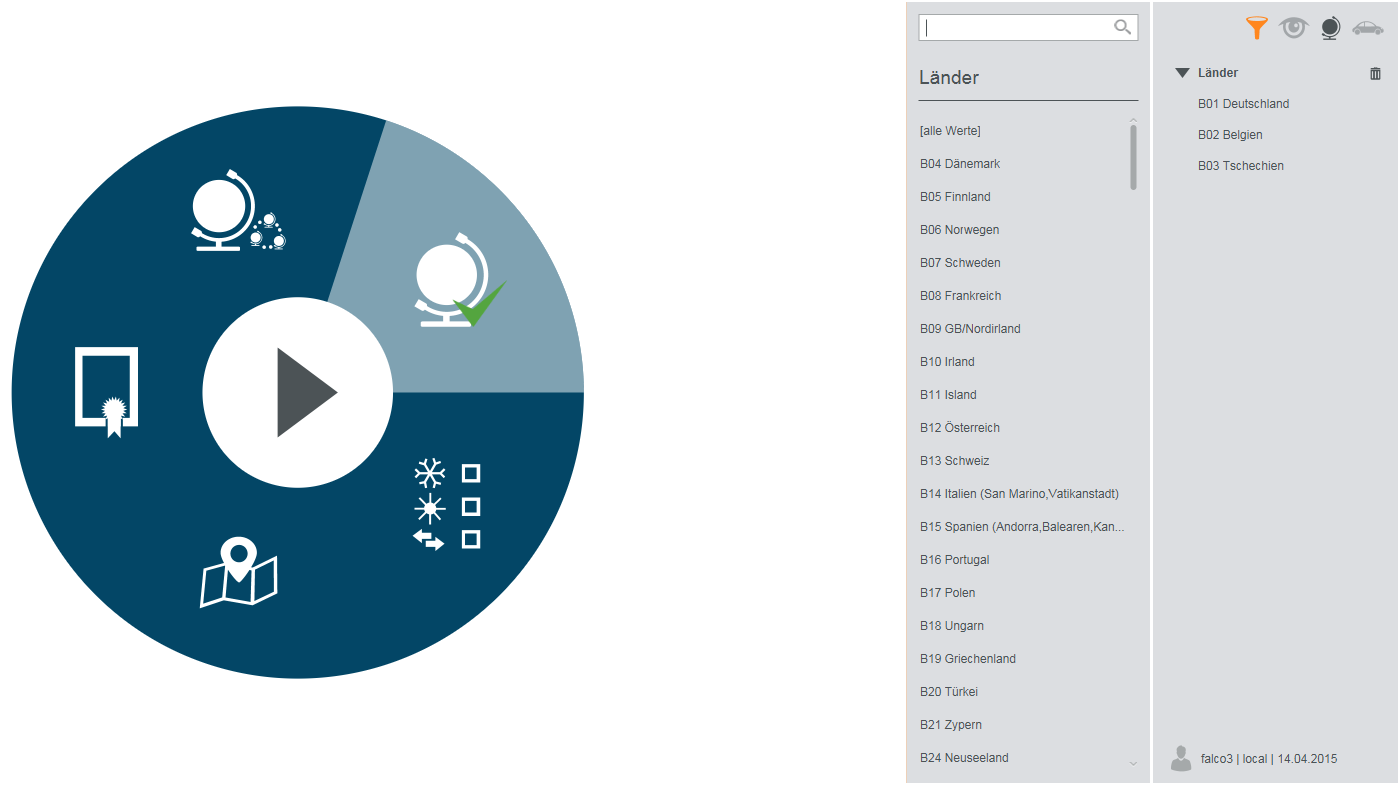
\includegraphics[width=0.6\textwidth]{grafiken/filter_short.png}
 \caption{Beispiel Filter}
 \label{fig:filter}
\end{figure}
Im Radial-Menü sind die Elemente kreisförmig um einen \textit{Play}-Button angeordnet, der standardmäßig deaktiviert ist. Erst, wenn die Ergebnismenge, die durch die gefilterten Attributwerte erzeugt wird, valide ist, wird der Button und das dazugehörige Navigationselement in der Navigationsleiste aktiviert. Die aktuelle Selektion in dem Menü wird durch einen helleren Kreisausschnitt über dem entsprechenden Element markiert. So wird dieser Bereich deutlich hervorgehoben.\par
Die Multi-Level-Liste enthält Werte, die als Filterkriterium ausgewählt werden können. Einige dieser Werte gruppieren weitere Werte und können nicht übernommen werden. Stattdessen öffnet sich beim Auswählen dieser Elemente eine untergeordnete Ebene der Multi-Level-Liste. Diese besonderen Unterkategorien sind mit einem Pfeil markiert, der in die gleiche Richtung zeigt, in die auch die nachfolgende Animation zum Wechsel der Ebene verläuft.\par
\begin{figure}[H]
 \centering
 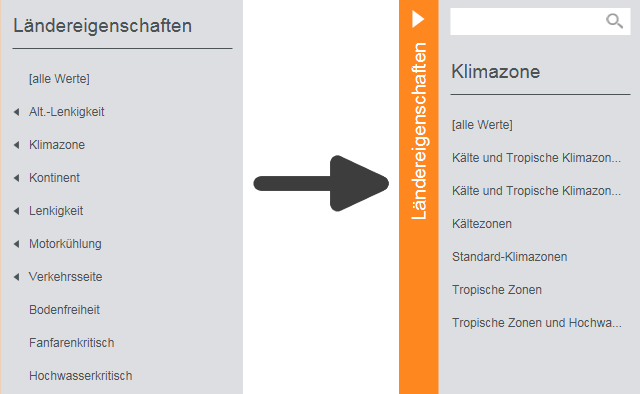
\includegraphics[width=0.4\textwidth]{grafiken/mll_combined.png}
 \caption{Multi-Level-Liste}
 \label{fig:mll}
\end{figure}
\subsection{Datendarstellung in Tabelle}
Nach dem Filtern der Daten lassen sich die Ergebnisansichten öffnen. Eine Präsentationsmöglichkeit ist die Tabellenansicht. Es handelt sich hierbei um eine komplexe Tabelle, die sämtliche Informationen darstellt. Die Spalten entsprechen den Attributen, zu denen erlaubte Werte im Filter ausgewählt wurden. Zusätzlich sind diese Attribute gruppiert. Die Trennung der Gruppen erfolgt durch deutlich sichtbare Linien, die vertikal zwischen den Spalten der einzelnen Gruppen verlaufen. Die einzelnen Gruppen lassen sich über Bedienelemente in der Sidebar aus- und einblenden, sowie per Drag \& Drop-Geste in der Reihenfolge vertauschen. Der um 45$^{\circ}$ geneigte Spaltenkopf sorgt für eine kompaktere Darstellung, da die minimale Spaltenbreite so nicht mehr durch den Titel der Spalte bestimmt wird. Besonders hilfreich ist diese Präsentation der Spaltenköpfe, wenn die zugehörigen Zellwerte nur sehr kurze Bezeichner annehmen. Der Beginn der gedrehten Beschriftungen ist dabei auf einer gedachten horizontalen Linie angeordnet. Auch in diesem Fall lässt sich das Gesetz der Kontinuität anwenden, wodurch die Überschriften als eine zusammengehörige Einheit wahrgenommen werden.\par
\begin{figure}[H]
 \centering
 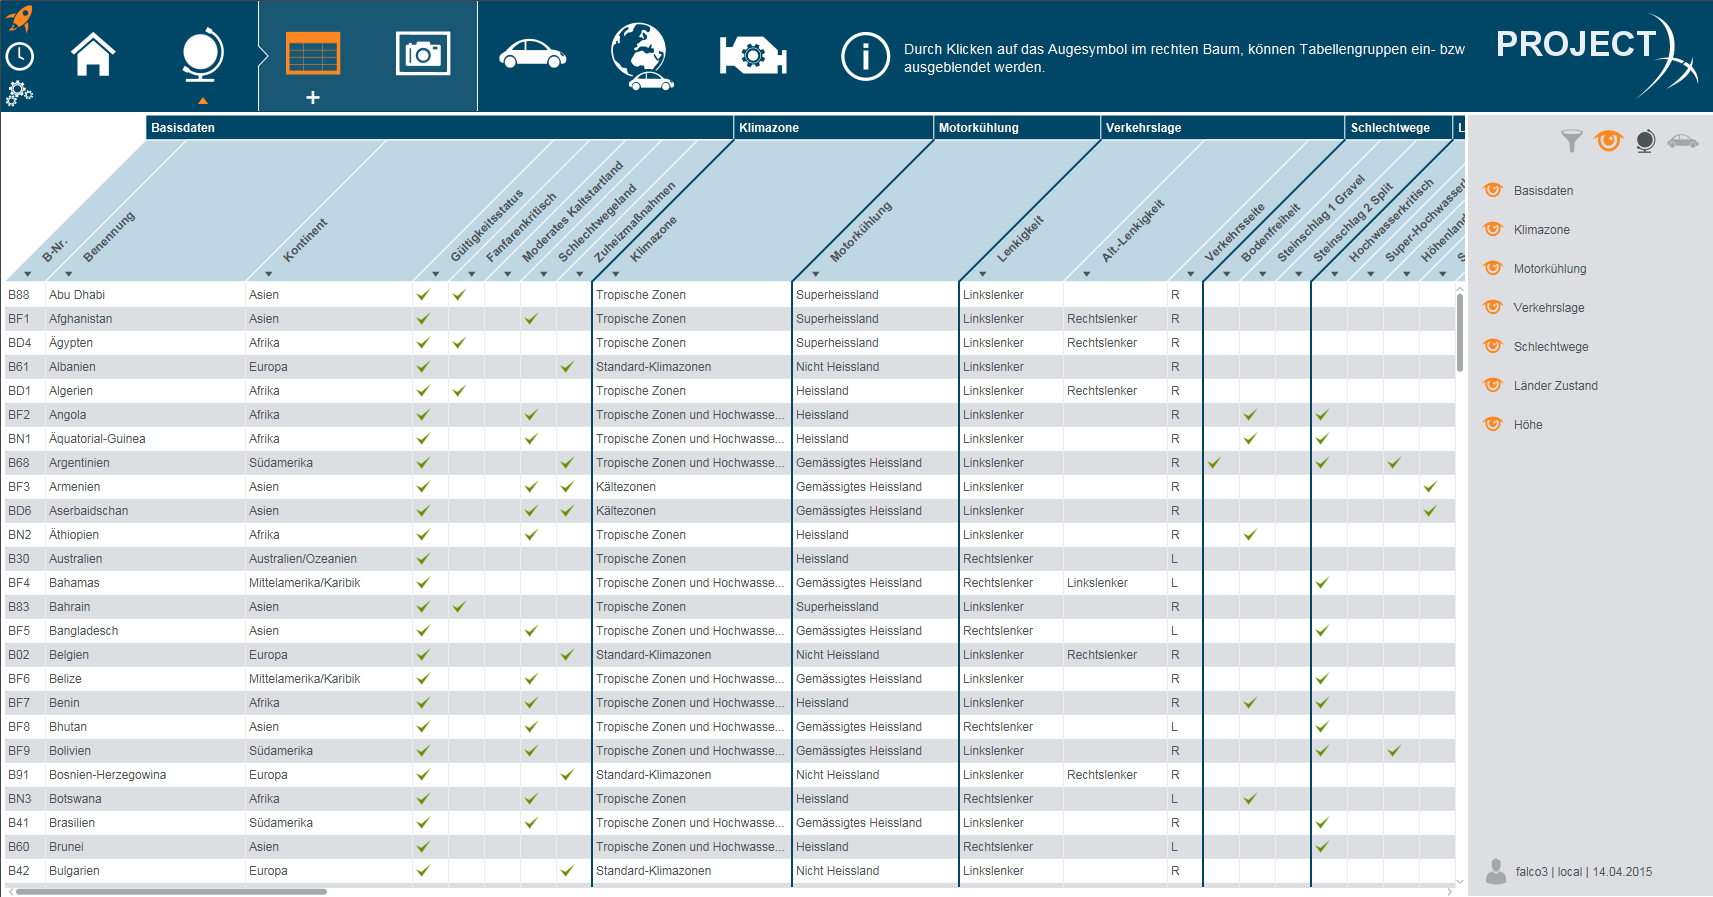
\includegraphics[width=0.7\textwidth]{grafiken/full_result_table.png}
 \caption{Ergebnistabelle}
 \label{fig:resultTable}
\end{figure}
Über die Pfeile im Spaltenkopf lässt sich ein \textit{Overlay} einblenden, in dem die präsentierten Daten auf einfache Weise zusätzlich eingeschränkt werden können. Zwar könnten die Pfeile als Elemente zur Umsortierung missverstanden werden, allerdings ist dies kein kritisches Problem, da sich das Overlay nach kurzer Zeit (oder nach dem Verlassen des Bereiches mit dem Mauscursor) schließt und andere Schaltflächen während der Anzeige nicht blockiert werden.\par
\begin{figure}[H]
 \centering
 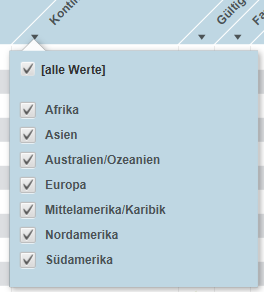
\includegraphics[width=0.3\textwidth]{grafiken/overlay.png}
 \caption{Schnellfilter-Overlay}
 \label{fig:autofilter}
\end{figure}
%Im Navigationsbereich ist unter der Schaltfläche der Ergebnispräsentation ein zusätzliches Icon (\ding{58}) aufgetaucht. Bei Klick auf den Bereich des zusätzlichen Icons öffnet sich, mit einer \enquote{Aufklapp-} Animation ein untergeordnetes Menü, das erweiterte Optionen für die derzeit aktive Ansicht bereitstellt. Darunter fallen die Export-Möglichkeiten in PDF und Excel. Die Animation verdeutlicht die Zugehörigkeit zu dem Menüpunkt des aktuell ausgewählten Elements.\par
\subsection{Datendarstellung in Galerie}
Eine weitere mögliche Ergebnispräsentation ist die Galerie. Hier werden im oberen Bereich Vorschaubilder für Daten angezeigt und darunter eine Detailansicht zum aktuell ausgewählten Element. Mit der Hilfe von $\blacktriangleright$ - und $\blacktriangleleft$ - Schaltflächen lassen sich die Objekte animiert durchschalten. Die aktuelle Selektion wird dadurch verdeutlicht, dass sich das entsprechende Element stets mittig über der Detailansicht befindet. Zusätzlich wird ein Bezeichner in orangener Schrift darüber angezeigt und das Element wird durch Vergrößerung hervorgehoben. Alle anderen Elemente rücken durch eine geringe Opazität, also einer geringeren Deckkraft, in den Hintergrund. Das Gesetz der Prägnanz wird hier durch mehrere ausschlaggebende Faktoren erfüllt und zeigt dem Anwender unmissverständlich die aktuelle Selektion an.\par
\begin{figure}[H]
 \centering
 \setlength{\fboxsep}{0pt}
 \setlength{\fboxrule}{0.5pt}
 \fbox{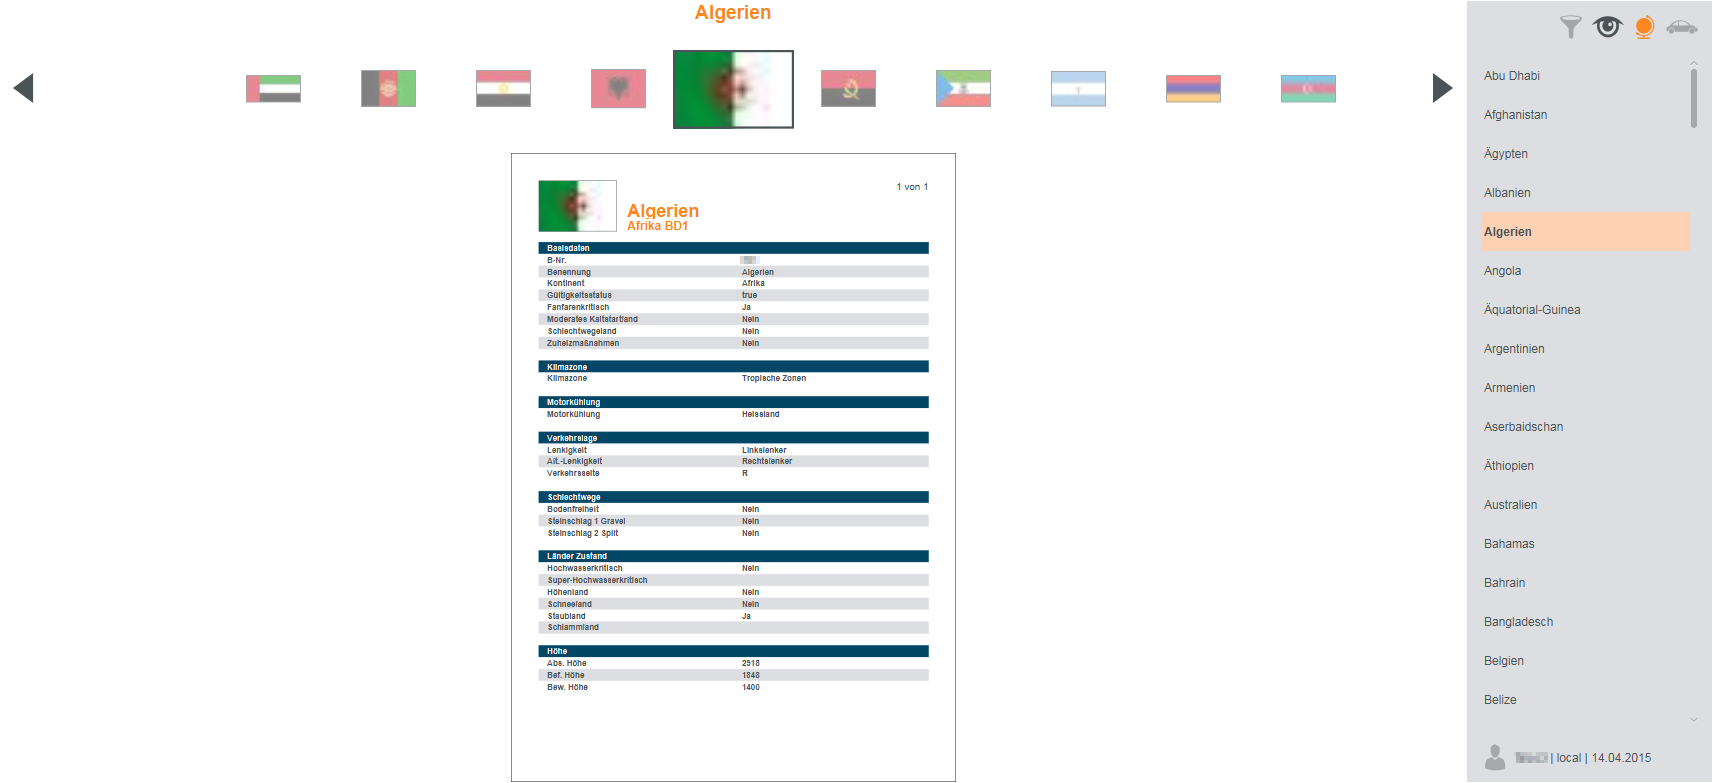
\includegraphics[width=0.7\textwidth]{grafiken/gallery.png}}
 \caption{Galerie}
 \label{fig:gallery}
\end{figure}
Für diese Ansicht ist in der Sidebar standardmäßig die \textit{Ergebnisvorschau} eingeblendet. Diese Ansicht bietet einen Überblick über alle Datensätze, die den Filterkriterien entsprechen. Die Selektion in dieser Liste ist mit der Selektion der Galerie-Komponente gekoppelt und wird synchron gehalten. Auch die \textit{Ansichtskonfiguration}, die bereits aus der Tabellenansicht bekannt ist, kann hier angewählt und verändert werden. Daraufhin ändern sich die in der Detailansicht der Galerie dargestellten Attributgruppen.\par
Ein Klick auf die Detailansicht öffnet eine vergrößerte Darstellung, den sogenannten \textit{Lesemodus}. Er bietet die Möglichkeit, die zuvor dargestellten Informationen durch die größere Darstellung besser lesen zu können. Die vorherigen und nachfolgenden Datensätze werden durch perspektivisch verschobene Seiten links und rechts der aktuell selektierten Seite eingeblendet. Durch Anklicken lassen sich diese, ebenfalls animiert, in den Vordergrund holen, während die aktive Seite \enquote{wegblättert}. Im Hintergrund verändert sich das selektierte Element in der Galerie. Durch das Anklicken des selbsterklärenden Tür-Icons in der unteren rechten Ecke lässt sich der Lesemodus wieder schließen.\par
\begin{figure}[H]
 \centering
 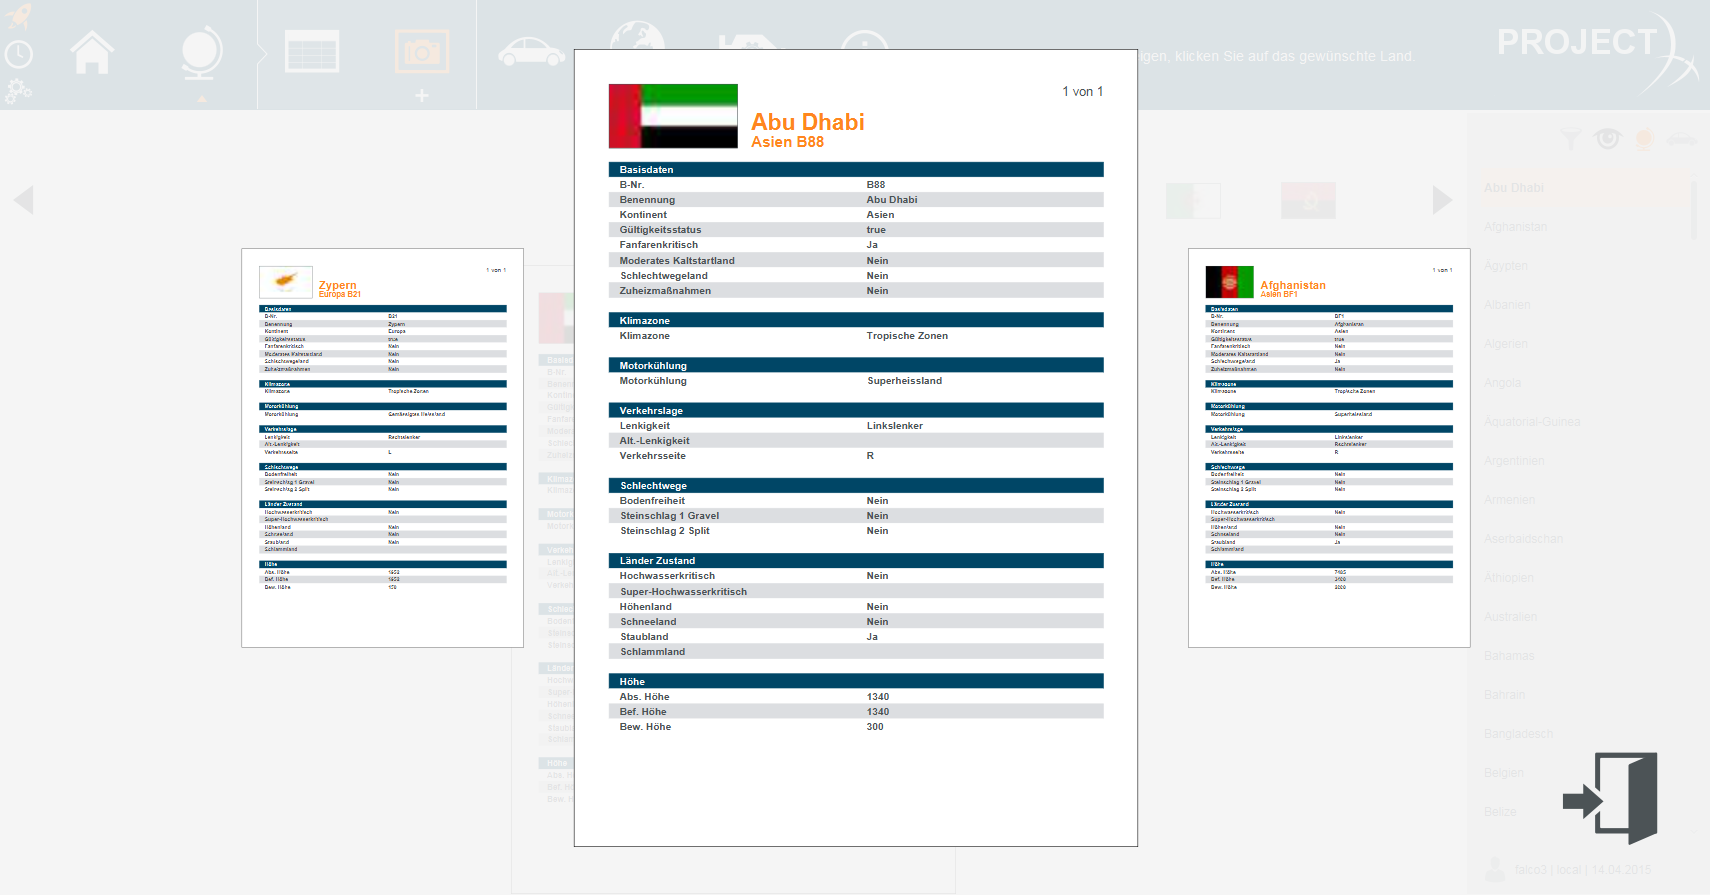
\includegraphics[width=0.6\textwidth]{grafiken/readmode.png}
 \caption{Lesemodus}
 \label{fig:readmode}
\end{figure}
\subsection{Darstellung kombinierter Daten}
Für den Anwendungsfall zur Darstellung kombinierter Länder- und Fahrzeugdaten gibt es spezialisierte Filter- und Ergebnisansichten. Der Filter muss verschiedene Modelobjekte verwalten um die Daten der kombinierten Ergebnismenge anzeigen zu können. Daher existieren zwei unterschiedliche Filter-Menüs, die sich mittels Buttons umschalten lassen. Die Buttons sind so gestaltet, dass sie der schematischen Darstellung des RadialMenüs entsprechen und ein Piktogramm der zugrundeliegenden Objekttypen enthalten. So besitzen auch diese Elemente eine Selbsterklärungsfähigkeit.
\begin{figure}[H]
 \centering
 
\includegraphics[width=0.2\textwidth]{grafiken/filter_buttons.png}
 \caption{Filter umschalten}
 \label{fig:filterButtons}
\end{figure}
Die Ergebnispräsentation in diesem Anwendungsfall unterscheidet sich von der der anderen Anwendungsfälle. In der Ergebnistabelle werden die Daten in einer \textit{Matrixdarstellung} visualisiert. Die Zeilen werden zu Beginn mit den konfigurierbaren Informationen der Fahrzeugdaten befüllt. Danach werden weitere Spalten erstellt, die mit den einzelnen Ländern aus den gefilterten Länderdaten gekennzeichnet sind. Auf diese Weise ergibt sich eine Matrix aus Daten für jede mögliche Fahrzeug-Länder-Kombination. Durch die unterschiedliche Gestaltung des Spaltengruppenkopfes heben sich die Länderspalten von den Spalten mit den Fahrzeugattributen visuell ab und definieren so einen eigenen Abschnitt.
\begin{figure}[H]
 \centering
 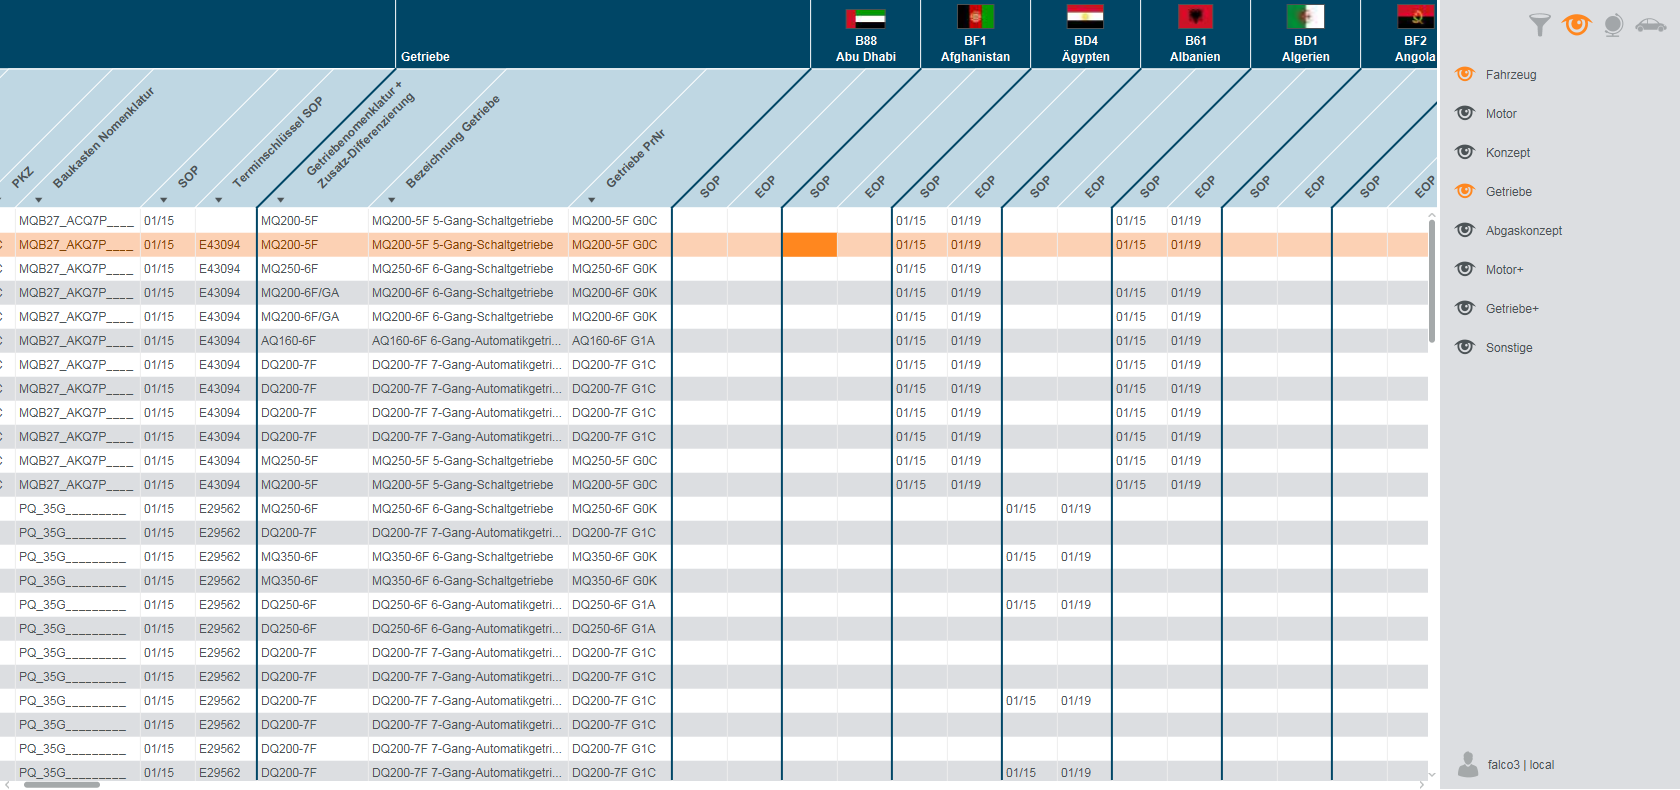
\includegraphics[width=0.6\textwidth]{grafiken/ltue_table.png}
 \caption{Matrix Ergebnistabelle}
 \label{fig:ltueTable}
\end{figure}
Die Selektion findet zellenweise statt. Durch einen Doppelklick auf eine einzelne Zelle können Details eingeblendet werden. Dennoch wird die Hintergrundfarbe der gesamten Zeile, in der sich die Selektion befindet, angepasst, damit die Orientierung in der komplexen Tabelle erleichtert wird. Das aktuell selektierte Fahrzeug ist so stets erkennbar, selbst, wenn die selektierte Zelle nicht sichtbar ist.\par
Die Detailansicht zu einer Datenkombination wird, anders als beim Lesemodus, nur im Content-Bereich der Applikation angezeigt. Hier wird für die Darstellung der Informationen weit weniger Platz benötigt, weshalb diese Darstellungsform ausreicht. Die Navigations- und die Seitenleiste sind weiterhin sichtbar, allerdings ist in der Sidebar keine Ansicht auswählbar und so wird diese leer angezeigt. Der Vorteil an der kontinuierlichen Sichtbarkeit der Navigationsleiste ist, dass der Kontext nicht verloren geht. Der Nutzer weiß also immer, wo er sich befindet, und welche Ansicht angezeigt wird, wenn er die Detailansicht wieder verlässt. Dies ist wichtig, da sowohl von der Tabellenansicht als auch von der Listenansicht, der weiteren verfügbaren Ergebnispräsentation, zu den Details navigiert werden kann.\par
\begin{figure}[H]
 \centering
 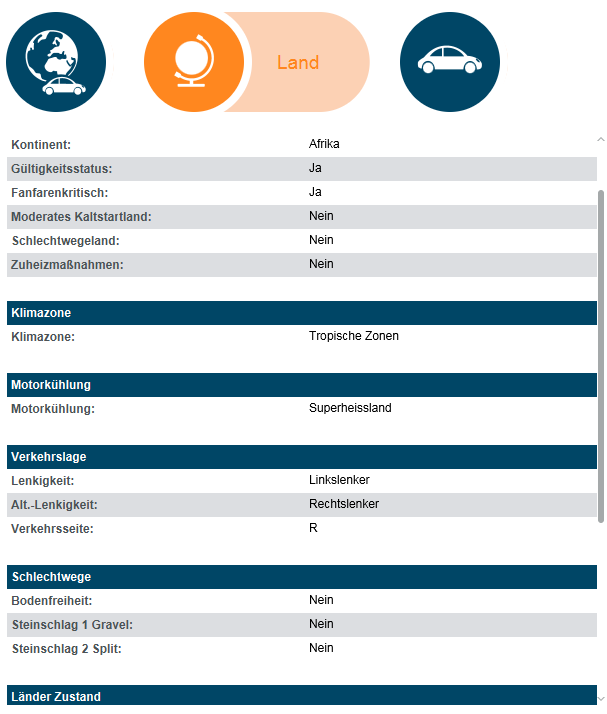
\includegraphics[width=0.3\textwidth]{grafiken/ltue_details.png}
 \caption{Detailansicht}
 \label{fig:ltueDetails}
\end{figure}
Die Listenansicht ist eine zweigeteilte Darstellung. Auf der linken Seite befindet sich eine Tabelle mit den Fahrzeugen der Ergebnismenge als Inhalt. Auf der rechten Seite werden alle gefilterten Länder angezeigt, zu denen für das links ausgewählte Fahrzeug Daten existieren. Da der Inhalt der linken Tabelle deutlich umfangreicher ist, nimmt diese Seite mehr Platz ein als die Länderliste. Durch Doppelklick auf das entsprechende Land können die Details eingesehen werden.\par
\begin{figure}[H]
 \centering
 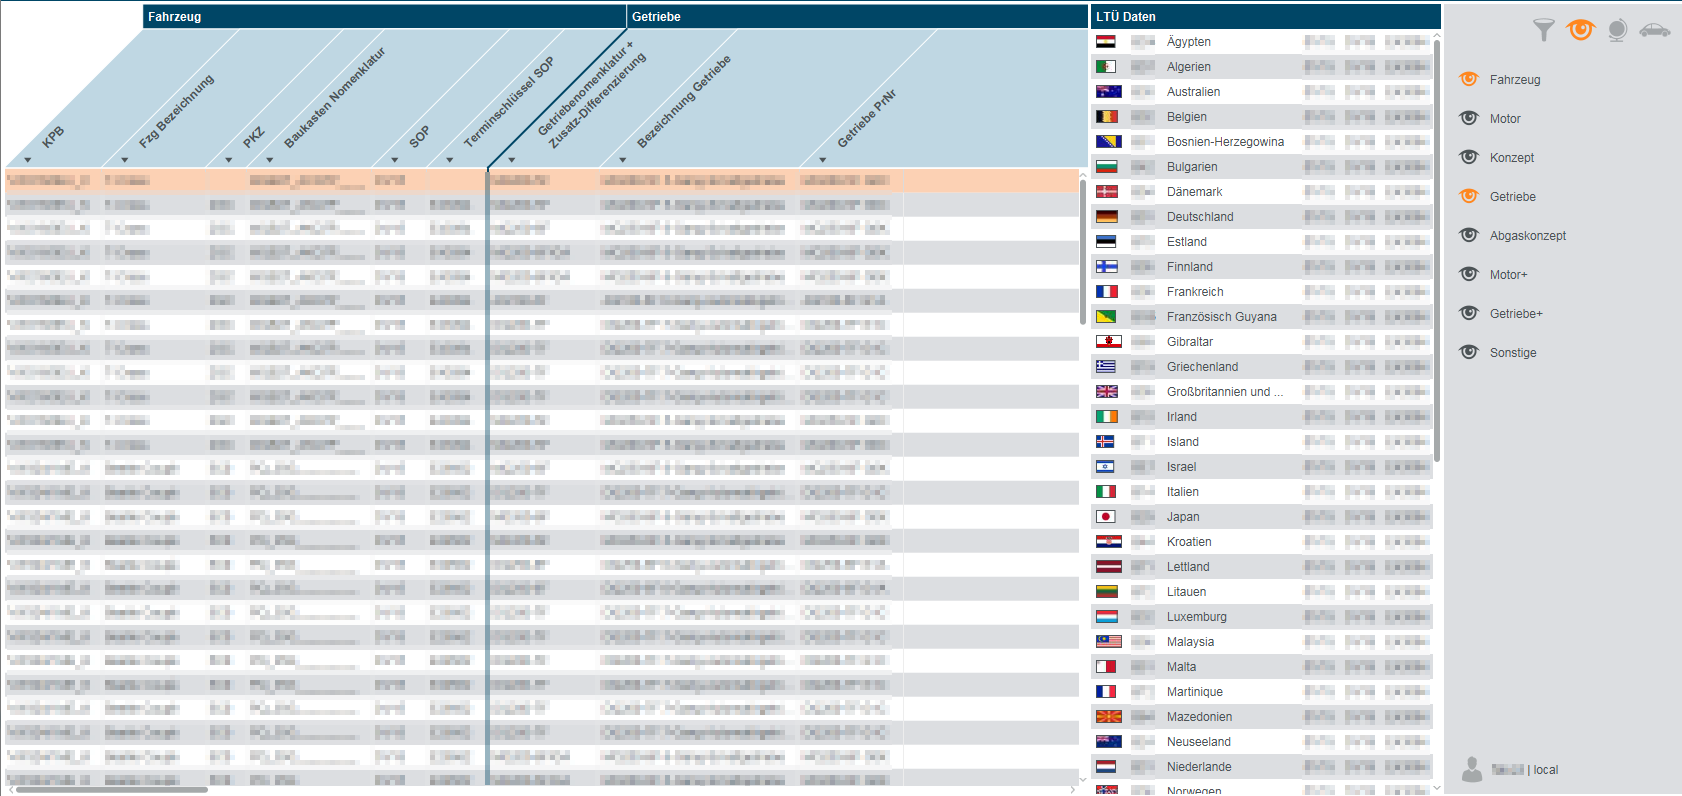
\includegraphics[width=0.6\textwidth]{grafiken/ltue_list.png}
 \caption{Listenansicht}
 \label{fig:ltueList}
\end{figure}
Durch die Ähnlichkeit der beiden Komponenten wird die Zusammengehörigkeit schnell deutlich. Dieser Effekt wird zum einen durch die gleich gestalteten Zeilen erwirkt (Wechsel zwischen weißer und grauer Zeile) und zum anderen durch die aneinander ausgerichteten Kopfelemente. Dies sind der Spaltengruppenkopf der Tabelle und die \enquote{Überschrift} der Länderliste.\par
\subsection{Tastaturbedienbarkeit}
Die Anwendung ist momentan nur per Maus steuerbar. Die Möglichkeiten der Tastatur, die an jedem Arbeitsplatz zu finden ist, werden nicht ausgenutzt - allein die Texteingabe über die Tastatur wird durch JavaFX voll unterstützt. Die Identifikation der Anwendungsbereiche, in denen die Tastatur eine alternative Bedienmöglichkeit darstellen kann, ist Ziel dieses Abschnittes. Dabei wird ein grundlegendes Konzept entworfen, für das in Abschnitt \ref{sec:designInteraction} spezialisierte Designlösungen gefunden werden.\par
Die erste Komponente, für die eine Tastatursteuerung denkbar wäre, ist die Navigation. Dabei sollten sowohl die Schaltflächen für das Umschalten der Navigationsleiste, als auch die Elemente per Tastatur bedienbar sein. So ist die grundlegende Steuerung der Anwendung möglich. Für die einzelnen Bildschirme müssen jeweils spezialisierte Lösungen gefunden werden.\par
Der erste Bildschirm, zu dem navigiert werden kann, ist in jedem Anwendungsfall der Filter. Hier gibt es das Radialmenü, die mehrstufige Liste und die Sidebar mit den gewählten Filterkriterien. Primär sollte die Liste mit der Tastatur bedient werden können, mit dem Ziel, Werte möglichst schnell zu finden und auszuwählen. Weiterführend kann die Steuerung für das Radialmenü umgesetzt werden, damit die Werte über verschiedene Attribute hinweg per Tastatur auswählbar sind. Die Bedienung der Sidebar ist eher nachrangig, da ihr Zweck ist, ausgewählte Werte wieder deselektieren zu können - folglich \enquote{nur} ein Mittel, um Fehler zu korrigieren.\par
In der Tabellenansicht, die in jedem Anwendungsfall verfügbar ist, ist eine Steuerung der Selektion denkbar. Außerdem sollte von einem Element zu den dazugehörigen Details gesprungen werden können, ohne dabei zur Maus wechseln zu müssen. Eine Steuerung der Sidebar wäre nur für den Reiter der Ansichtskonfiguration von Nöten, da die anderen verfügbaren Ansichten nur der Ergebnisvorschau dienen.\par
Ähnlich ist die Situation bei der Galerie. Auch hier wäre eine Tastatursteuerbarkeit der Galerie, inklusive Öffnen der vergrößerten Ansicht im Lesemodus vorteilhaft. Das Durchschalten der Elemente kann ebenfalls mit der Tastatur erfolgen. Das Konzept dafür sollte nach Möglichkeit in allen Ergebnispräsentationen ähnlich sein. So sollte auch der Lesemodus nach dem gleichen Schema behandelt werden.\par
%Bei der Detailansicht, die von der Ergebnistabelle und der Listenansicht erreichbar ist, ist eine Unterstützung der Subnavigation (Wechsel zwischen LTÜ-, Land- und Fahrzeugdaten) in diesem Bildschirm denkbar.\editHere{Wenn hier, dann auch in Impl}\par
\subsection{Übertragung von Touchgesten auf Maussteuerung} \label{sec:analyseGesten}
Mit Blick auf den immer stärker werdenden Trend, auch Geschäftsanwendungen auf mobile Geräte zu portieren, soll an dieser Stelle geprüft werden, inwiefern die Touchgesten (vgl. Kapitel \ref{fig:touchGestures}) auf das Bedienkonzept am Desktop-PC übertragbar sind. Dies soll zum einen zu einer intuitiveren Bedienung mit der Maus beitragen und zum anderen für die Benutzung der Software auf Convertibles vorsorgen.\par
Der Mauszeiger wird zu diesem Zweck als \enquote{Ersatz} für den Finger auf einem Touch-Display verwendet. Da es nur einen Mauszeiger und eine Maus gibt, ist es technisch gesehen nur möglich, Gesten durchzuführen, die genau einen Finger benötigen. Dies sind \textit{Tap}, \textit{Double Tap}, \textit{Drag}, \textit{Flick} und \textit{Press} (vgl. Abb. \ref{fig:touchGestures}). Die \textit{Tap} und \textit{Double Tap}-Gesten entsprechen sowohl von der Durchführung, als auch von der Semantik in der Regel dem einfachen Mausklick bzw. dem Doppelklick. Die \textit{Drag}-Geste ist der Drag \& Drop Aktion der Maus sehr ähnlich. An vielen Stellen jedoch, an denen bei mobilen Anwendungen \textit{Drag}-Gesten verwendet werden würden, wird die Benutzung eines UI-Elements auf dem Desktop-PC mit anderen Mitteln gelöst. Für den \textit{Flick}, auch \textit{Swipe} genannt, existiert kein Pendant im Pensum der Standardinteraktionen durch Maus- und Tastatureingaben. Dennoch ist es denkbar, eine solche Geste mit einer schnell ausgeführten Drag \& Drop-Aktion zu ermöglichen. Auch der \textit{Press} kann mit den gegebenen Eingabemitteln umgesetzt werden. Eine solche Aktion ist jedoch in den meisten Fällen nur bedingt intuitiv verwendbar, da keine ähnlichen, dem Nutzer vertrauten, Aktionen für die Maussteuerung existieren. Als Ersatz kann der Rechtsklick bei der Desktop-Verwendung genutzt werden.\par
Die erste Komponente, für die eine Gesten-Unterstützung untersucht wird, ist die Navigationsleiste. Hier ist jedes aktive Element durch einen einfachen Mausklick verwendbar. Dieses Verhalten entspricht dem, was Nutzer mobiler Anwendungen bei der Bedienung erwarten würden. \textit{Swipe} oder \textit{Drag}- Gesten würden hier eher zu Verwirrung führen.\par
Die Bedienung des Radialmenüs im Filter ist zunächst nur mit einfachen Klicks auf die Zielelemente möglich. Als Alternative dazu sollten auch Touchgesten und deren Pendant auf Desktop-PCs bereitgestellt werden. Bei der Bedienung der Liste wird sich bislang auf das Scrollrad und den Scrollbalken verlassen. Auf Geräten, die nativ Toucheingaben unterstützen, ist das Scrolling per \textit{Drag} durch das UI-Toolkit bereits unterstützt. Um das Verhalten auf verschiedenen Plattformen anzugleichen und die Spanne von unterstützten Eingabemethoden zu erhöhen, sollte die Bedienmöglichkeit auch für die Maus umgesetzt werden. Durch diese Art von Scrolling kann vorallem in langen Listen genauer und zielgerichteter zu gesuchten Einträgen gelangt werden.\par %Sidebar?
In den Ergebnisansichten, in denen eine Tabelle bzw. eine Liste verwendet wird, stellt sich ein vergleichbares Problem. Jegliche Art von Tabelle oder Liste kann mit einer \textit{Drag}-Geste gescrollt werden, wenn die Eingabe über ein Touch-Display erfolgt. Die Steuerung sollte auch an diesen Stellen an die Touch- Bedienung angepasst werden. Dies sind im Speziellen die Ergebnistabelle und die Listenansicht.\par
In der Galerie muss die Umsetzung auf eine eigene Weise erfolgen. Die Leiste, in der die Vorschaubilder der angezeigten Datensätze angezeigt werden, kann ebenfalls mit neuen Bedienungsmöglichkeiten versehen werden, um die aktuelle Selektion zu verändern. Eine Steuerung, die nur über die Buttons links und rechts der Bordüre abgehandelt wird, schränkt den Nutzer stark ein. Ein ähnliches Verhalten zeigt der Lesemodus. Hier lässt sich das zentrierte, vergrößerte Datenblatt nur durch Anklicken eines der seitlichen Datenblätter ändern.\par
%Zu guter Letzt existiert noch eine tabellenartige Komponente in der Detailansicht. Werden in der Komponente genügend Daten angezeigt, muss auch diese per Gesten gescrollt werden können.\par
\section{Design} \label{sec:designInteraction}
Nachdem die relevanten Stellen in der Analysephase aufgedeckt wurden, werden in diesem Abschnitt konzeptionelle Lösungen entwickelt, nach denen die Umsetzung erfolgen kann.\par
\subsection{Tastaturbedienung} \label{sec:interactionKeyboard}
Das Implementieren der einzelnen Teillösungen ist nicht sinnvoll, ohne zunächst ein Gesamtkonzept entworfen zu haben. Wie in der Analysephase festgestellt, gibt es mehrere Komponenten, für die eine Tastaturbedienung ermöglicht werden soll. Einige dieser Komponenten können zeitgleich auf dem Bildschirm sichtbar sein (z.B. die Navigationsleiste und die mehrstufige Liste der Filteransicht). Das führt in der Bedienung zu Konflikten, da Tastatureingaben, nach dem in Abschnitt \ref{sec:javafxEventhandling} beschriebenen Event-Handling-Konzept, nur an einem spezifischen Knoten im Szenegraphen angelangen, wenn dieser den Eingabefokus besitzt. Es ist demnach nicht möglich, die Events an einem bestimmten Knoten zu behandeln indem der Fokus auf dieses Element gesetzt wird. Das Problem kann jedoch umgangen werden. Anstatt EventHandler an den jeweiligen Komponenten zu registrieren, können die EventHandler direkt an dem \textit{Szene}-Knoten, also der Wurzel des Szenegraphen, angemeldet werden.\par
\heading{Sekundäre Funktionalitäten}
Ein Konzept, das in modernen Anwendungen oft Verwendung findet sind die \textit{Mnemonics} (vgl. Kap. \ref{sec:inputDevices}). Diese werden häufig durch das einmalige Drücken der \textit{Alt}-Taste visualisiert, das die Einblendung der möglichen Tastenkombinationen zufolge hat. Eine ähnliche Umsetzung kann für die Sekundärfunktionen erfolgen. Dazu zählen vor allem die Navigationsleiste und die Sidebar. Um den Nutzer dabei zu unterstützen, die mit Mnemonics versehenen Elemente zu identifizieren, wird (bei Drücken der \textit{Alt}-Taste) über der gesamten Anwendung eine teil-transparente Ebene eingeblendet, die genau die Stellen ausspart, an denen sich steuerbare Objekte befinden. Zudem wird in den dadurch erzeugten Bereichen die Tastenkombination eingeblendet, welche die entsprechende Aktion ausführt.\par
Für das Steuern der Navigationsleiste eignen sich die Zahlentasten am besten. Die verschiedenen Navigationsleisten werden parallel dazu mit den Funktionstasten F1, F2, etc. umgeschaltet. Die Ähnlichkeit und Nähe der Tasten zueinander sowie deren Anordnung sorgen für eine intuitive Bedienbarkeit. Um die Sidebar zu bedienen sollten im Optimalfall sprechende Kombinationen gewählt werden. Das wäre beispielsweise der Buchstabe \enquote{E} für Ergebniskonfiguration oder \enquote{F} für die Filterauswahl. Generell gilt: Es sollten nur die Elemente mit Mnemonics versehen werden, die sichtbar, aktiv und auch mit normalen Mausklicks zu verwenden sind.\par
\heading{Filterbildschirm}
Die Haupteingabe findet immer in dem derzeit im Content-Bereich aktiven Bildschirm statt. Unter diese Bildschirme fällt der Filter. Die damit primär durchgeführte Aktion ist das Auswählen von Attributwerten aus der mehrstufigen Liste. Zu der Liste gehört stets das Schnellfilter-Textfeld im oberen Bereich. Der normale Arbeitsablauf eines Nutzers ist das Anklicken des Textfeldes, Eingeben eines Textes und Anklicken des gefundenen Wertes. Um diesen Ablauf möglichst effizient zu gestalten sollte der Wechsel von Tastatur zu Maus erspart werden. Dies kann erreicht werden, indem die Eingabe eines Zeichens immer dazu führt, dass das Textfeld den Fokus erhält und der Text dort eingegeben wird, unabhängig davon, welches Element den Fokus derzeit besitzt. Diese Umsetzung ist nur möglich, weil parallel keine weiteren Elemente existieren, die eine direkte Eingabe von Text erwarten oder den Eingabefokus benötigen. Weitergehend können die Pfeiltasten der Tastatur für die Navigation in der Liste genutzt werden. Hat der Nutzer einen Text eingegeben und möchte einen gefundenen Wert selektieren, kann er von der Eingabe mit der $\downarrow$- Taste direkt zum ersten Element der Liste springen und darin auf natürliche Weise weiter navigieren. Zu einer untergeordneten Ebene kann mit der $\leftarrow$- Taste gelangt werden und die entgegengesetzte Aktion, das zurückspringen zur übergeordneten Ebene, wird durch $\rightarrow$ bereitgestellt.\par
Die Bedienung des Radialmenüs wird durch die globale Eingabe im Textfeld und die Verwendung der Pfeiltasten für die Liste zwar eingeschränkt, aber auch hier kann das erwähnte Konzept der Mnemonics nach dem gleichen Schema wie in der Navigation verwendet werden. Zwar ist das Radialmenü Teil des angezeigten Bildschirms, gemessen an der Benutzungshäufigkeit ist die Multi-Level-Liste jedoch ein höher priorisiertes Bedienelement. Das Verhalten ist dahingehend konsistent mit dem Gesamtkonzept der Steuerung.\par
\heading{Ergebnisansichten}
Die Ergebnisansichten sollten intuitiv mit den Pfeiltasten der Tastatur steuerbar sein. Bei Zeilenselektion haben nur die $\downarrow$- und $\uparrow$- Tasten einen Effekt. Ist die Zellselektion aktiviert, können die $\leftarrow$- und $\rightarrow$- Tasten für die Navigation durch die Spalten genutzt werden. Würde sich die nächste per Pfeiltaste selektierte Zelle außerhalb des angezeigten Bereiches befinden, muss die Tabelle entsprechend gescrollt werden. Die Enter-Taste kann dazu verwendet werden, um die dem Anwendungsfall entsprechende Detailansicht des angewählten Datensatzes aufzurufen.\par
Die Galerie kann durch verschiedene Tastatureingaben unterstützt werden. Zum einen kann, genau wie in der Ergebnistabelle, per Pfeiltasten zwischen den Elementen gewechselt werden, zum anderen können aber auch Freitext-Eingaben zu einer intuitiven Bedienung beitragen. Ist der Galerie-Bildschirm aktiv, kann der Nutzer anfangen, einen Text zu tippen. Solange die Tastendrücke nicht zu lange auseinander liegen, wird der Text mit dem Wert des primären Attributes aller Datensätze verglichen. Anhand des Länderanwendungsfalles würde dies bedeuten, dass der Anwender nach einem bestimmten Land sucht. Anstatt dieses aus der langen Länderliste heraussuchen zu müssen, kann er den Anfang des Namens eintippen und die Galerie scrollt automatisch zu dem gesuchten Element. Ist der Nutzer also auf der Suche nach dem Land \enquote{Deutschland}, tippt er \enquote{Deu} und gelangt noch während des Tippvorganges zu dem Datensatz. Auch hier öffnet die Enter-Taste wiederum die Detailansicht, die in diesem Anwendungsfall durch den Lesemodus repräsentiert wird.\par
Konsistent zu den anderen Ansichten lässt sich im Lesemodus der im Fokus stehende Datensatz mit den Pfeiltasten durchschalten. Drücken der ESC-Taste schließt den Lesemodus erwartungsgemäß. \par
Eine komplett identische Umsetzung dieses Konzeptes ist in der Listenansicht nicht möglich. Hier gibt es zwei Komponenten, die mit den Pfeiltasten bedient werden müssen. Der Bedienungsablauf ohne Tastatursteuerung wäre der, dass der Nutzer zunächst ein Fahrzeug aus der Tabelle auswählt. Daraufhin werden ihm in der rechtsseitigen Liste alle Länder angezeigt, die zu den Filtereinstellungen passen und für die eine Daten existieren. Zwischen der Bedienung dieser beiden Teile der Darstellung sollte gewechselt werden können. Dies kann zum Beispiel durch die $\leftarrow$- und $\rightarrow$- Tasten gelöst werden. Standardmäßig sollte jedoch die linke Hälfte der Ansicht im Fokus der Bedienung stehen.\par
%Die Subnavigation der LTÜ-Detailansicht kann unter Verwendung der Pfeiltasten ($\leftarrow$- und $\rightarrow$) bedient werden. Die Selektion würde erwartungsgemäß von e
\subsection{Gestensteuerung}
Das Ziel der Gestensteuerung ist es, dem Nutzer eine intuitive Bedienung der Oberflächenelemente zu ermöglichen. Durch die in Abschnitt \ref{sec:analyseGesten} erläuterten Gesten ist es möglich, die Anwendung auf verschiedenartigen Geräten auf die gleiche Weise zu benutzen. Dabei kann zwischen bereichsabhängigen Gesten (z.B. \textit{Drag}) und unabhängigen Gesten (z.B. \textit{Swipe}) unterschieden werden.
\heading{Filterbildschirm}
In der Filteransicht sollte sowohl das Radialmenü, als auch die mehrstufige Liste unterstützt werden. Zusätzlich zu der Bedienung des kreisförmigen Menüs durch einfache Klicks, können hier \textit{Drag}-Aktionen für eine unkomplizierte Bedienung sorgen. Auf Mobilgeräten ist es häufig möglich, diese Selektion durch eine Geste, statt durch \textit{Tap}s zu ändern. Die Geste beginnt über dem Abschnitt des Menüs, der selektiert ist und wird bis zu dem Abschnitt ausgeführt, der das Ziel darstellt. Dabei ist der Weg der Geste unerheblich und die Selektion folgt ihr. Für eine optimale Erfahrung sollte die Position des Selektionsbereiches nicht abhängig von der Entfernung des Mauszeigers bzw. des Fingers vom Mittelpunkt des Menüs sein. Alleine der Winkel vom Start der Geste bis zum Ziel oder derzeitigen Berührungspunkt/ der derzeitigen Mauszeigerposition ist hierfür ausschlaggebend:\par
\begin{figure}[H]
 \centering
 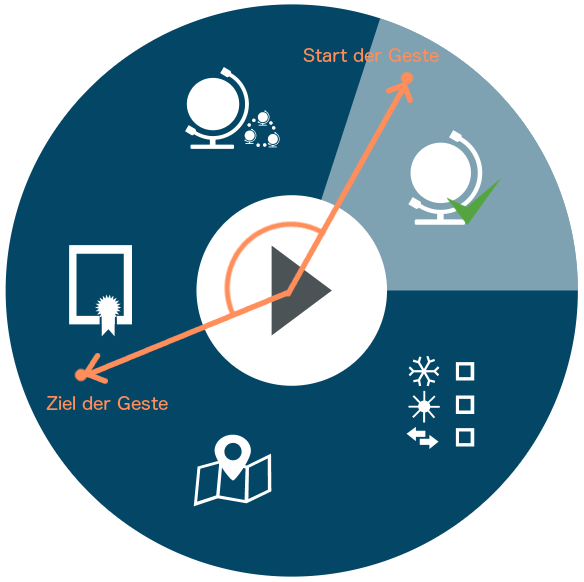
\includegraphics[width=0.45\textwidth]{grafiken/radial_gesture.png}
 \caption{Radialmenü Geste}
 \label{fig:radialGesture}
\end{figure}
Der hell eingefärbte Kreisausschnitt muss sich also um genau den Winkel, der in der beispielhaften Abbildung \ref{fig:radialGesture} zu sehen ist, um den Mittelpunkt des Kreises drehen. Bei jeder Bewegung der Maus sollte die Position des Selektionsbereiches aktualisiert werden. Nach Abschließen der Geste erhält der Menüeintrag die Selektion, in dessen Teilbereich die Winkelhalbierende des Selektions-Kreisausschnittes liegt - also jenes Element, welches zu einem größeren Teil durch den hell eingefärbten Kreisausschnitt bedeckt wird. Dabei wird der Kreisausschnitt durch eine Animation so positioniert, dass er wieder exakt über dem selektierten Element liegt. \par
Für die Liste kann eine \textit{Drag}- Geste zum Scrollen eingeführt werden, die analog zu der nativ vorhandenen mobilen Geste funktioniert. Das bedeutet, die Liste folgt der vertikalen Bewegung des Mauszeigers bzw. des Fingers.\par
\heading{Ergebnisansichten}
Für alle Tabellen und Listen innerhalb der Ergebnisansicht kann das gleiche Konzept angewandt werden, das bereits für die mehrstufige Liste des Filters entworfen wurde. Bei Tabellen muss zusätzlich zu der vertikalen Verschiebung, die horizontale Änderung der Mauszeiger- oder Fingerposition beachtet werden. Die Vorschaubilder in dem Galerie-Bildschirm können ebenfalls als eine Art Liste gesehen werden, welche die Elemente horizontal nebeneinander ausrichtet. Daher sollte auch diese Komponente durch \textit{Drag}-Gesten unterstützt werden. Bei Vollendung der Aktion muss zu dem Element gesprungen werden, das dem Mittelpunkt, also der Stelle, an der stets das selektierte Element angezeigt wird, am nächsten liegt. Dieses Verhalten ist konsistent mit dem Verhalten des Radialmenüs im Bezug auf die Gestenunterstützung und sorgt so für einen höheren Wiedererkennungswert und eine gute Lernförderlichkeit.\par
Im Lesemodus eignen sich \textit{Swipe}-Geste am besten, um ein gestengestütztes Selektieren zu ermöglichen. Die \textit{Swipe}-Geste ist bei vielen mobilen Anwendungen vertreten, in denen Informationen mehrseitig visualisiert werden. Führt man die Geste von links nach rechts aus, wird die linke Seite in den Vordergrund gerückt, von rechts nach links ist das Verhalten umgekehrt. Der Unterschied zum \textit{Drag} ist der, dass die zurückgelegte Strecke des Swipes unerheblich für die Aktion ist und keine kontinuierlichen Aktualisierung erforderlich ist. Es wird nach Abschluss der Geste genau eine Aktion ausgeführt. Diese ist in dem Fall das Umblättern der Seite.\par
\section{Implementierung} \label{sec:interactionImplementation}
\subsection{Globale Eingabeerkennung}
Um die Tastatureingaben des Nutzers behandeln zu können, unabhängig davon, welches Element gerade den Eingabefokus besitzt, wird eine globale Eingabeerkennung benötigt. Das theoretische Konzept dafür wurde bereits in Kapitel \ref{sec:interactionKeyboard} vorgestellt. In der Praxis ist es jedoch schwierig, an verschiedenen Stellen der Anwendung EventHandler an der Szene anzumelden. Dafür wird zunächst das Szene-Objekt benötigt. Jeder Knoten im Szenegraphen bietet die Funktion \textit{\#{}getScene()}, welche die Szene zurückliefert. Dies funktioniert aber nur, wenn das UI-Objekt bereits im Szenegraphen integriert ist. Dies ist in der Regel nicht der Fall, wenn die Komponente erst noch aus einzelnen Objekten zusammengestellt wird. Aus diesem Grund wurde ein Manager entworfen, der genau einen EventHandler an der Szene registriert. An diesem Manager, auf den über den \textit{Context} zugegriffen werden kann, werden wiederum \textit{Consumer} registriert, an die das Event direkt weitergeleitet wird. Der \textit{Context} ist ein Objekt, dass einige Funktionen statisch verfügbar macht. Zu jedem Zeitpunkt ist höchstens ein \textit{Consumer} aktiv, der die Tastatur-Events erhält. Das Registrieren eines weiteren \textit{Consumers} führt zur Deaktivierung des vorherigen. So ist sichergestellt, dass die Events nur an genau einer Stelle bearbeitet werden.\par
\subsection{Mnemonics mit Overlay}
Die Umsetzung dieses Konzeptes gliedert sich in mehrere Teilprobleme:
\begin{enumerate}
 \item Das Finden und Erkennen der Knoten, die Mnemonics unterstützen
 \item Die Umsetzung der Tastaturkürzel
 \item Das Konstruieren und Einblenden des Overlays
\end{enumerate}
Das Finden der betroffenen UI-Elemente kann auf zwei Weisen gelöst werden. Die erste Möglichkeit ist, dass sich jeder Knoten bei einem Manager registriert, der alle unterstützten Knoten mit deren Tastaturkürzeln verwaltet. Die andere Möglichkeit ist das Suchen nach jenen Komponenten, die Mnemonics unterstützen. Der Vorteil der ersten Methode ist die Performanz, da bereits alle notwendigen Knoten bekannt sind. Auf der Gegenseite sind dadurch gravierende Veränderungen an dem vorhandenen Quellcode von Nöten, da die Komponente nur zu der Zeit aktiv bzw. an dem Manager registriert sein darf, zu der sie die gegebene Aktion auch unterstützt. Dies erfordert ein dynamisches An- und Abmelden des UI-Objektes. Die zweite Methode hingegen ist weniger invasiv. Zwar muss der Szenegraph mit Hilfe eines Suchalgorithmus traversiert werden, dies nimmt aber selbst bei vielen Elementen vernachlässigbar wenig Zeit in Anspruch. Daher ist dies die bevorzugte Variante. Als Erkennungsmerkmal und zur Bereitstellung der notwendigen Informationen implementieren die Klassen der benutzerdefinierten Komponenten ein Interface. Wird die Alt-Taste gedrückt, durchsucht ein Breitensuchalgorithmus den Szenegraphen und findet alle Knoten, die das Mnemonic-Interface implementieren.\par
Das Interface gibt außerdem durch eine Methode \textit{\#{}getCode} Aufschluss darüber, welches Tastenkürzel für diesen Knoten vorgesehen ist. Mit JavaFX wurde auch die Klasse \textit{Mnemonic} eingeführt. Der Konstruktor der Mnemonic-Klasse erwartet einen JavaFX-Node als Übergabeparameter, auf den ein \textit{ActionEvent} abgefeuert wird, sobald das Mnemonic ausgelöst wird. Damit ein Mnemonic ausgelöst werden kann, muss es zunächst unter Angabe einer Tastenkombination an der Szene registriert werden. Das Problem bei der Verwendung dieses Konzeptes ist, dass die Knoten, die bedient werden sollen, keine \textit{ActionEvent}s behandeln. Sie reagieren ausschließlich auf \textit{MouseClicked}- Events. Anstatt das Verhalten jeder einzelnen Komponente zu ändern und sie für \textit{ActionEvent}s anzupassen, kann das Verhalten des Mnemonics durch Ableitung verändert werden. Es muss lediglich die Methode \textit{\#{}fire} überschrieben werden. Anstatt ein \textit{ActionEvent} abzufeuern, wird dadurch in der neu erstellten Klasse \textit{ClickMnemonic} ein \textit{MouseClicked}- Event für den Zielknoten synthetisiert. Für jeden durch den Suchalgorithmus gefundenen Knoten lässt sich so ein \textit{ClickMnemonic} an der Szene registrieren, sobald die Alt-Taste gedrückt wird und wieder abmelden, wenn sie erneut gedrückt wird.\par
Das Overlay, welches irrelevante bzw. nicht bedienbare Elemente überdeckt, wird unter Verwendung einer bereits vorhandenen API gelöst. Diese Schnittstelle erlaubt es, beliebige Elemente über den anderen Elementen der Benutzeroberfläche einzublenden (vgl. Abb. \ref{fig:readmode}). Der Knoten, der die anderen Objekte überlagert, ist ein halb durchsichtiges, weißes Rechteck, das an den Stellen, unter denen sich bedienbare Elemente befinden, \enquote{Löcher} hat. Diese besondere Form kann mit einer JavaFX-Methode erzeugt werden, die Objekte vom Typ \textit{Shape} von einem anderen Objekt des selbigen Typs \enquote{subtrahiert}. Dabei werden Positionierungs- und Rotationsinformationen beachtet. Es wird also ein neues Shape erzeugt, das nur aus den Teilen der beiden Formen besteht, die sich nicht überlagern.\par
Damit das Overlay korrekt funktionieren kann, wird für jedes UI-Element, dass Mnemonics unterstützen möchte, ein Shape benötigt, das genau die Form dieses Knotens haben sollte. Auch diese Information kann über das bereits entworfene Interface bereitgestellt werden. Eine statische Hilfsmethode in diesem Interface konvertiert beliebige rechteckige Knoten in ein solches Shape. Eine weitere Methode führt eine vergleichbare Operation für kreisförmige Elemente aus. Andersförmige Knoten müssen diese Berechnung selbstständig implementieren. Die Shapes, die dadurch von allen Mnemonic-unterstützenden Knoten zusammenkommen, fungieren als eine Art Schablone, aufgrund der das rechteckige Overlay \enquote{ausgestanzt} wird. Aus diesem Grund ist das Interface \textit{IMnemonicStencilProvider} benannt.\par
Abschließend werden zusätzlich zu dem Overlay Labels eingeblendet, welche dem Nutzer die Tastenkombination für die einzelnen Elemente anzeigen. Die Berechnung dafür findet ebenfalls im \textit{IMnemonicStencilProvider} innerhalb einer default Methode statt und entspricht standardmäßig der oberen linken Ecke des Ausschnittes:\par
\needspace{7\baselineskip}
\begin{lstlisting}[
    language=Java,
    caption=IMnemonicStencilProvider\#{}getLabelPosition,
    label=getLabelPosition]
    default Point2D getLabelPosition() {
        return new Point2D(getStencil().getLayoutX(), getStencil().getLayoutY());
    }
\end{lstlisting}
Die abstrakte Implementierung erlaubt es auf einfache Weise beliebigen Komponenten, wie der Navigationsleiste, dem Radialmenü oder Teilen der Sidebar, Mnemonics zu unterstützen. Für das Umschalten der Navigationsleiste werden die Funktionstasten F1 bis F3 vergeben, die Navigationsitems selbst können per Zahlentaste 1 bis 9 (und 0) bedient werden. Das Radialmenü erhält die Tastenkombination, ebenso wie die Seitenleiste abhängig von dem Attributnamen des Elementes (bspw. L für Land, M für Motor). Ist der erste Anfangsbuchstabe bereits vergeben, wird der nächstmögliche, folgende genommen. Das Prinzip ist das gleiche bei der Ergebniskonfiguration der Seitenleiste. Hier werden die Anfangsbuchstaben der Attributgruppen als Tastenkürzel gewählt.\par
\begin{figure}[H]
 \centering
 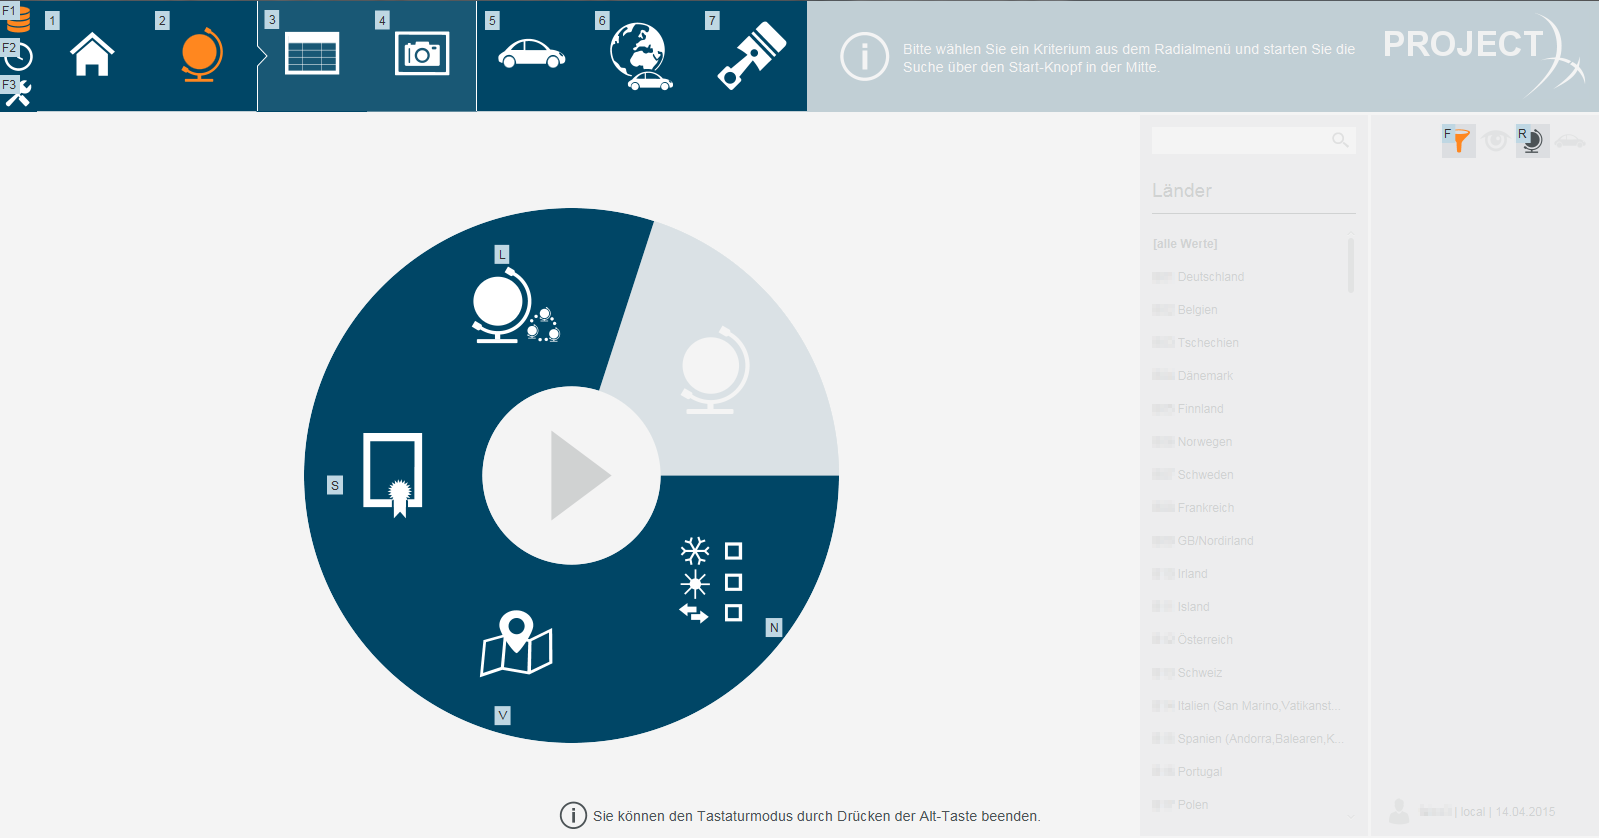
\includegraphics[width=0.85\textwidth]{grafiken/mnemonics.png}
 \caption{Mnemonics mit Overlay}
 \label{fig:mnemonicsOverlay}
\end{figure}
\subsection{Filter}
In der Filteransicht muss die Gestensteuerung für die Multi-Level-Liste und das Radialmenü umgesetzt werden, sowie eine Tastaturunterstützung für die Liste. Die zuvor implementierten Mnemonics decken die Tastatursteuerung für das Radialmenü bereits ab. Das Prinzip ist hier analog zu der Seitenleiste. \par
Bei der Umsetzung des Scrollings für die mehrstufige Liste können verschiedene Ansätze verfolgt werden. Der nächstliegende ist das manuelle Implementieren der Drag- Geste. Dazu muss bei Erkennung einer Drag-Aktion auf der Liste, die Scroll-Position des Inhaltes kontinuierlich, auf Basis der vertikalen Änderung der Mauszeigerposition, aktualisiert werden. Dies ist nur möglich, indem die die Position der Scrollbalken modifiziert wird. Ein anderer, subtilerer Ansatz besteht darin, der ListView vorzugaukeln, die verwendete Hardware sei Touch-fähig und das MouseEvent würde durch eine Toucheingabe hervorgerufen werden. Obwohl dieser Ansatz zunächst komplizierter klingt, ist der erforderliche Aufwand geringer. Einige JavaFX-Komponenten, die eine dynamische Anzahl an Elementen verwalten müssen, bestehen mitunter aus einem sogenannten Flow. Der Flow verwaltet, am Beispiel der ListView, alle Listenelemente und ist für das Scrollen zuständig. Er enthält eine Variable, die initial gesetzt wird, die das \enquote{Panning} verwaltet und bei der Erstellung gesetzt wird. Bei einem Computer ohne Touch-Display ist diese Variable standardmäßig auf \textit{false}, kann aber nachträglich modifiziert werden. Ist die Variable auf \textit{true} gesetzt, reagiert die Liste auf eine Drag-Geste mit der Maus genauso wie auf eine Geste per Toucheingabe.\par
Die Gestenunterstützung für das RadialMenü kann nicht auf die gleiche Weise implementiert werden. Hier wird die Berechnung manuell umgesetzt. Dafür wird ein EventHandler an dem UI-Element angemeldet, das den Kreisausschnitt der aktuellen Selektion darstellt. Der EventHandler reagiert auf das Event \textit{DRAG\_{}DETECTED} und initialisiert daraufhin einige JavaFX-Properties, die für die Berechnung der neuen Position des Selektionsausschnittes benötigt werden. Dies sind die Start-Koordinaten des Drag-Events, sowie die derzeitige Mauszeigerposition. Die Mauszeigerposition wird daraufhin bei jeder Bewegung der Maus aktualisiert und entspricht so immer dem aktuellen Wert. Auch hierfür ist ein EventHandler erforderlich (vom EventTyp \textit{MOUSE\_{}DRAGGED}). Ein weiteres Property ist durch das JavaFX Binding-Konzept über eine Berechnung an die aktuellen und die Start-Koordinaten gebunden. Durch die Berechnung hat dieses Property immer einen Double-Wert zwischen 0 und 360, der der Position des Kreisausschnittes entspricht. Für die Dauer der Geste wird die Position des Kreisausschnittes an den Wert der Berechnung gebunden. Wird die Maustaste wieder losgelassen, werden die Werte zurückgesetzt. Die Positionsberechnung geschieht wie folgt:\par
\begin{lstlisting}[
    language=Java,
    caption=Berechnung Startposition des Kreisausschnittes als Winkel,
    label=getLabelPosition]
    DoubleExpression targetAngle = Bindings.createDoubleBinding(() -> {
            Point2D arcCenter = localToScene(selectionArc.centerXProperty().get(), selectionArc.centerYProperty().get());
            Point2D start = new Point2D(startX.get(), startY.get());
            Point2D current = new Point2D(currentX.get(), currentY.get());

            double value = arcCenter.angle(start, current);
            // determine angle direction (for angles > 180 degree)
            if (start.subtract(arcCenter).crossProduct( current.subtract(arcCenter)).getZ() > 0) {
                value = 360 - value;
            }
            value = (startAngle.get() + value) % 360;
            return value;
        }, startAngle, currentX, currentY);
\end{lstlisting}
Für die Tastatursteuerung der Liste kann die zuvor vorgestellte Schnittstelle zur globalen Eingabeerkennung genutzt werden. Wenn ein Eingabeevent von dem Consumer verarbeitet wird, wird zunächst geprüft, ob es sich um ein \textit{KEY\_{}PRESSED}- oder \textit{KEY\_{}TYPED}-Event handelt. Ein \textit{KEY\_{}TYPED}-Event wird immer dann ausgelöst, wenn ein Unicode-Character eingegeben wurde, wird eine der Funktionstasten, Pfeiltasten o.ä. gedrückt, wird ein \textit{KEY\_{}PRESSED}-Event ausgelöst. Eine Grobfassung des Algorithmus ist folgend dargestellt:\par
\begin{figure}[H]
 \centering
 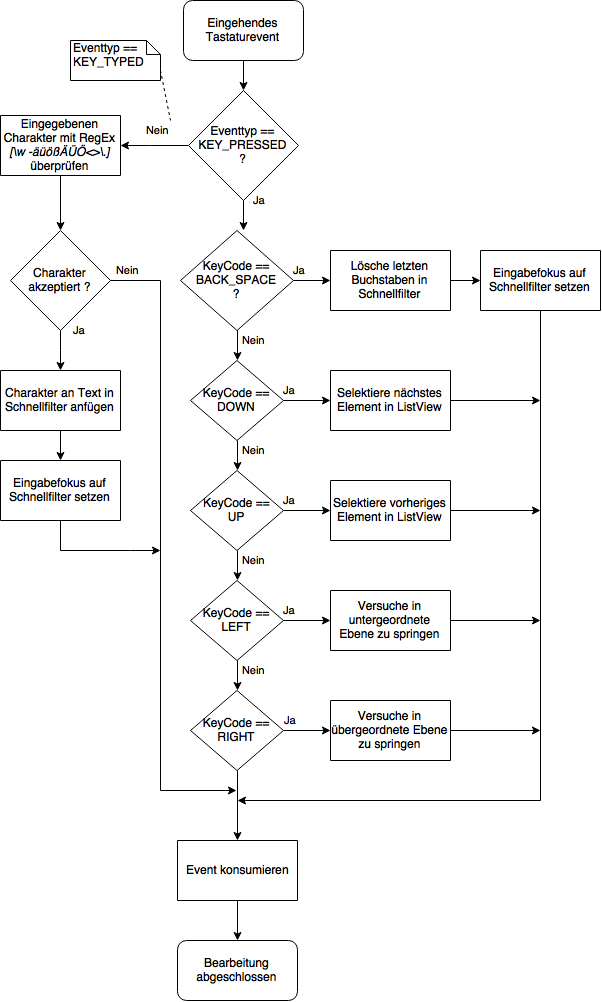
\includegraphics[width=0.75\textwidth]{grafiken/MLL_KeyCapture.png}
 \caption{Multi-Level-Liste Tastatursteuerung}
 \label{fig:mllKeyCapture}
\end{figure}
Einige Implementierungsdetails sind in dem Schaubild nicht aufgeführt, spielen aber für das grundlegende Konzept keine tragende Rolle. Wird ein Zeichen eingegeben, wird zunächst mit Hilfe eines regulären Ausdruckes gefiltert, ob das entsprechende Zeichen akzeptiert wird. Ist dies der Fall, wird das Zeichen direkt in das Textfeld des Schnellfilters eingegeben und der Fokus darauf gesetzt. Handelt es sich um einen \enquote{normalen} Tastendruck (der keinem Unicode-Charakter zugeordnet ist) wird auf Basis einer Fallunterscheidung jeweils eine zugeordnete Aktion ausgeführt.\par
Schwierigkeiten traten beim automatischen Scrolling auf, das ausgelöst werden muss, sobald die Selektion außerhalb des sichtbaren Bereiches gesetzt wird. Die nativ implementierte Scroll-Funktion ermöglicht es nur, eine bestimmte Zelle zum Anfang des \textit{ViewPorts}, also des sichtbaren Bereiches zu scrollen. Ein solches Verhalten ist ungewöhnlich und dementsprechend nicht intuitiv verwendbar. Daher muss eine weitere Berechnung durchgeführt werden, durch die erschlossen werden kann, welches Listenelement an die erste Stelle gescrollt werden muss, damit die gerade selektierte Zelle in den sichtbaren Bereich gelangt.\par
\subsection{Ergebnisansichten}
Wie auch bei der mehrstufigen Liste in der Filteransicht, kann die Drag-Geste für die verschiedenen Tabellen und Listen der Ergebnisansichten über das Panning realisiert werden, welches normalerweise das Scrollen auf Touch-Geräten ermöglicht. So sind nur geringfügige Eingriffe in den vorhandenen Code nötig.\par
Das Steuern der Galerie mit Drag-Aktionen ist vergleichbar mit der Implementierung im Radialmenü. Anstatt jedoch eine Winkelberechnung zwischen Start- und derzeitiger Position der Geste durchzuführen, wird nur die horizontale Änderung betrachtet und daraufhin die Verschiebung der Vorschauleiste auf der X-Achse berechnet. Auch hier werden wieder verschiedene Properties für die Berechnung der Verschiebung genutzt. So hat es den Anschein, als würde der Nutzer die Bordüre der Vorschaubilder von einer Koordinate zu einer anderen ziehen können. Mit Abschluss der Aktion wird die Position der Leiste per Animation korrigiert, sodass das Element, welches dem Mittelpunkt des sichtbaren Teils der Leiste am nächsten ist, ausgewählt wird.\par
\begin{figure}[H]
 \centering
 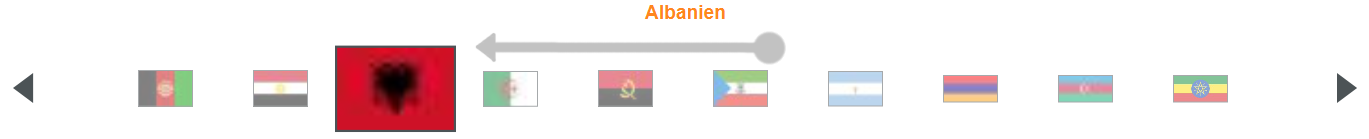
\includegraphics[width=0.75\textwidth]{grafiken/gallery_drag.png}
 \caption{Galerie Gestensteuerung}
 \label{fig:mllKeyCapture}
\end{figure}
Im Lesemodus wird statt einer Drag-Aktion die Umsetzung einer Swipe-Geste benötigt. Diese ist wiederum ähnlich aufgebaut wie die Drag-Aktion in der Galerie. Der Unterschied besteht darin, dass die Position der einzelnen Seiten im Lesemodus nicht konstant animiert werden muss.  Das bedeutet, eine Aktualisierung ist erst mit Abschluss der Geste erforderlich. Wird die Geste von links nach rechts ausgeführt, liegt eine positive Änderung der X-Koordinate von Start zu Zielpunkt der Geste vor. Dies resultiert in einem \enquote{Zurückblättern}, andernfalls in einem \enquote{Vorblättern}.\par
Die Unterstützung der Tastatur in den Ergebnistabellen ist konzeptionell parallel zu der Implementierung in der Multi-Level-Liste aufgebaut. Auch hier werden wieder Fallunterscheidungen für die verschiedenen akzeptierten Eingaben benötigt. Allerdings muss hier beim Wechsel der Selektion unterschieden werden, ob bei der Tabelle Zeilen- oder Zellselektion aktiviert ist. Bei Zellselektion muss zusätzlich zu dem vertikalen Scrollverhalten auch das horizontale Scrollverhalten nach dem gleichen Schema angepasst werden, damit das Konzept intuitiv verwendbar ist.\par
Die Eingabeunterstützung für die Galerie-Komponente besteht, ähnlich der Multi-Level-Liste, aus dem Teil, der die die \textit{KEY\_{}PRESSED}-Events behandelt und dem Teil, der die \textit{KEY\_{}TYPED}-Events behandelt. Die Fallunterscheidung der \textit{KEY\_{}PRESSED}-Events ist konsistent mit den anderen Ergebnisansichten und der Steuerung in der Filteransicht. Es werden also die Pfeiltasten (in diesem Falle $\leftarrow$ und $\rightarrow$) unterstützt, sowie die Enter-Taste zum Ausführen der assoziierten Aktion (hier: Öffnen des Lesemodus). Die Verarbeitung der Texteingabe funktioniert anders als im Filterbildschirm. Hier führt die Eingabe eines Zeichens dazu, dass eine Zeichenkette erstellt wird. Es wird sofort innerhalb der Bezeichnungen der Modellelemente, die in der Galerie angezeigt werden, nach dem ersten Eintrag gesucht, der mit der Zeichenkette beginnt. Anfänglich besteht die Zeichenkette nur aus einem Zeichen. Wird innerhalb von 500 Millisekunden ein weiteres Zeichen getippt, wird es an die Zeichenkette angefügt und die Suche wird erneut mit der verlängerten Zeichenkette ausgeführt. So ist es möglich, auch nach längeren Bezeichnern zu suchen, wenn einige Bezeichner mit den gleichen Anfangsbuchstaben beginnen. Erzielt die Suche einen Treffer, wird die Galeriekomponente zu dem entsprechenden Element gescrollt.\par
Der Lesemodus unterstützt diese Funktion bewusst nicht, da diese Ansicht für das \enquote{Blättern} entworfen wurde, nicht um nach den Details spezieller Elemente zu suchen. Für diese Funktionalitäten stehen die anderen Ergebnispräsentationen zur Verfügung. Wie bei den anderen Ansichten ist hier das Wechseln der Datenblätter per Pfeiltasten durch eine einfache Fallunterscheidung implementiert. \par